\chapter{Marco teórico} % (fold)
\label{cha:marco_teorico}



\section{Conversión Analógico-Digital y El conversor Delta-Sigma}
\label{sec:conversion_analogica_digital_y_el_conversor_delta_sigma}



\subsection{Conversion analogico digital} % (fold)
\label{sub:conversion_analogico_digital}
%CITADO

Para poder medir ciertos fenómenos naturales, se utilizan sensores físicos que miden las magnitudes de estos fenómenos y las traducen en tensiones voltaicas en la salida. Una lectura de dicha tensión nos da una idea de la magnitud física de lo que se esta midiendo. Si se obtiene, a partir de esta tensión, datos digitales que la representen, es posible construir un software que realice determinadas acciones en función de datos provenientes de los sensores. Un conversor analógico-digital es un dispositivo que toma como entrada una señal analógica voltaica, y la convierte en datos digitales.

La salida de los sensores, que permiten al equipo electrónico interaccionar con el entorno, es  normalmente  una  señal  analógica,  continua  en  el tiempo.  En  consecuencia,  esta información  debe  convertirse  a  binaria  (cada  dato  analógico  decimal  codificado  a  una palabra formada por unos y ceros) con el fin de adaptarla a los circuitos procesadores y de presentación. Un convertidor analógico-digital (CAD) es un circuito electrónico integrado cuya salida es la palabra digital resultado de convertir la señal analógica de entrada. \\

La conversión a digital se realiza en dos fases: cuantificación y codificación. Durante la primera se  muestrea la entrada y a  cada valor analógico obtenido se asigna un valor o estado, que depende del número de bits del CAD. El valor cuantificado se codifica en binario en una palabra digital, cuyo número de bits depende de las líneas de salida del CAD. Estos dos procesos determinan el diseño del circuito integrado. \\

En la práctica, el proceso de conversión está sujeto a numerosas limitaciones resultado de los procesos de fabricación. Las más relevantes son el tiempo de conversión y la finitud del número de estados de salida. La conversión involucra un tiempo y, en consecuencia, supone  una  incertidumbre  que  limita  la  velocidad  máxima  de  la  entrada.  Los  valores discretos  del  proceso  de  cuantificación  llevan  consigo  un  error  y  una  limitación  de resolución del circuito. La elección del CAD en un diseño electrónico dependerá de la adaptación de sus rasgos a  los requerimientos de la aplicación. \cite{adc}

% subsection conversion_analogico_digital (end)



\subsection{Conversores de canal único, de canal pseudo diferencial, y de canal totalmente diferencial}
\label{sub:conversores_de_canal_unico_de_canal_pseudo_balanceado_y_de_canal_totalmente_balanceado}
%CITADO

Un Conversor Analógico-Digital puede obtener la señal de voltaje de entrada mediante tres métodos distintos: Canal único, Canal pseudo diferencial, y canal totalmente diferencial. \\

En general, lo mas simple es elegir aquella estructura que sea compatible con el sensor que se utiliza. Pero a pesar de eso, existen ciertas características que reúne cada estructura que deben considerarse. Si existe un circuito de acondicionamiento de señal entre el sensor y el conversor, también puede afectar a la decisión sobre que tipo de estructura utilizar. Algunos conversores son configurables y permiten elegir entre canal único y pseudo diferencial, o canal único y totalmente diferencial.\cite{tipos_canales}

\subsubsection{Canal único}
\label{subs:canal_unico}

Las entradas de canal único son suficientes para la mayoría de las aplicaciones. En este tipo de estructuras, la señal de entrada tiene una referencia a la masa común del conversor. Esta masa es compartida por todas las entradas que estén configuradas en este modo. La Figura \ref{fig:canalunico} ilustra el muestreo de una señal para esta estructura.

A diferencia de las totalmente diferenciales, las entradas de canal único son mas sensibles al ruido y al desfasaje de continua. El desfasaje de continua (DC Offset) es un fenómeno que ocurre cuando el nivel de continua en la señal es distinto de 0. El ruido en el canal y el desfasaje de continua reducen la amplitud dinámica de la señal de entrada, lo cual provoca que la calidad de la conversión sea menor.\cite{dc_offset}

Este tipo de entradas suelen utilizarse en aquellos casos en que la fuente que produce la señal y el conversor A/D están cerca uno del otro (Por ejemplo, en la misma placa de cobre), y por lo tanto el desfasaje de continua y el ruido no son tan presentes como en casos donde estén mas separados. También se puede incluir un circuito que adapte la señal y reduzca estos efectos no deseados.\cite{tipos_canales}

\begin{figure}[h]
  \centering
  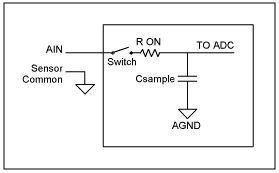
\includegraphics[width=0.60\textwidth, height = 4cm]{canalunico}
  \caption{Conversión de canal único. La señal se toma midiendo la tensión en el capacitor con respecto a una masa única compartida por todos los canales del conversor}\label{fig:canalunico}
\end{figure}

% subsubsection canal_unico (end)

\subsubsection{Canal totalmente diferencial}
\label{subs:canal_totalmente_diferencial}

Una entrada totalmente diferencial es la que mayor inmunidad al ruido presenta. Como puede verse en la Figura \ref{fig:totalmentediferencial}, cada una de las entradas esta conectada a un canal distinto del conversor. La medición final se calcula con la diferencia entre ambas entradas y no con respecto a masa, lo cual cancela el ruido entre ambas y elimina el desfasaje de continua. La desventaja de este conversor es que consume dos canales por cada señal en lugar de uno solo, como es en el caso de las estructuras de tipo canal único.\cite{tipos_canales}

\begin{figure}[h]
  \centering
  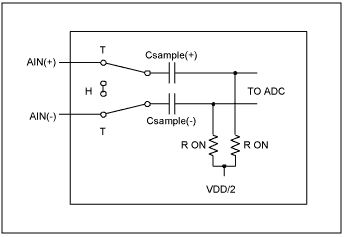
\includegraphics[width=0.80\textwidth, height = 6cm]{totalmentediferencial}
  \caption{Conversión totalmente diferencial. El valor que se mide esta dado por la diferencia entre ambas entradas, esto es lo que cancela el ruido presente en ambas señales, aumentando el rango dinámico de la conversión.}\label{fig:totalmentediferencial}
\end{figure}

% subsubsection canal_totalmente_diferencial (end)

\subsubsection{Canal pseudo-diferencial}
\label{subs:canal_pseudo_diferencial}

Las entradas pseudo-diferenciales son similares a las totalmente diferenciales en el hecho que separan la masa del conversor con la masa general, permitiendo que no haya desfasaje en continua en la señal. Pero no son una buena alternativa para eliminar ruido común.\cite{tipos_canales}


% subsubsection canal_pseudo_diferencial (end)

\subsection{Conversor Delta-Sigma} % (fold)
\label{sub:conversor_delta_sigma}

De manera básica, los conversores Delta-Sigma consisten en dos bloques: un bloque con un modulador Delta-Sigma, seguido de un bloque de filtro digital mas un decimador. El primer bloque aplica una técnica de muestreo de alta frecuencia a la señal analógica de entrada, produciendo a la salida una señal digital de 1 bit. El segundo bloque toma las muestras y las convierte en un código de menor frecuencia y mayor resolución. Existen dos frecuencias involucradas: La frecuencia de muestreo $f_s$ y la frecuencia de datos $f_d$. La Figura \ref{fig:deltasigma} muestra el diagrama de bloques de este conversor.\cite{delta_sigma_1}

\begin{figure}[h]
  \centering
  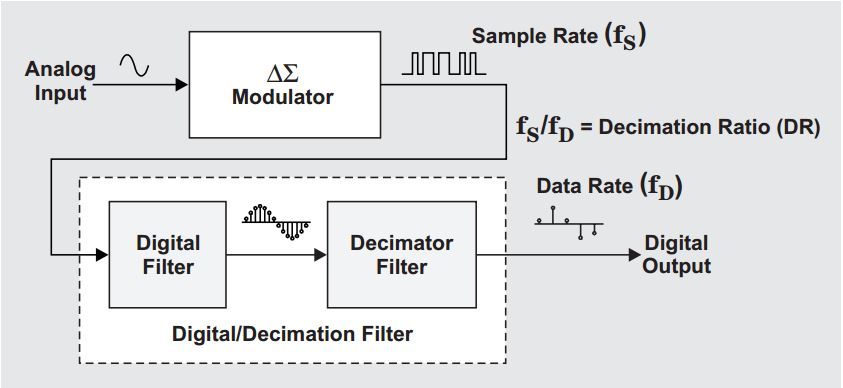
\includegraphics[width=0.80\textwidth, height = 6.3cm]{deltasigma}
  \caption{Diagrama de bloques del conversor analógico digital Delta-Sigma. El primer bloque corresponde al modulador Delta-Sigma, y el segundo al filtro digital con filtro de decimación}\label{fig:deltasigma}
\end{figure}

\subsubsection{El modulador Delta-Sigma} % (fold)
\label{ssub:el_modulador_delta_sigma}

El modulador Delta-Sigma es el responsable de digitalizar la señal de entrada y reducir el ruido en frecuencias bajas. La arquitectura del modulador implementa una técnica conocida como modelado de ruido, que empuja las frecuencias del ruido fuera de la banda de interés, reduciendo así el ruido en la señal convertida. Esto hace que los convertidores Delta-Sigma sean apropiados para casos donde se trabaja con señales de entrada de baja frecuencia y se requiere alta precisión en la medición. \\

El modulador convierte la señal de entrada en un tren de pulsos de un bit a la salida. La razón entre los unos y los ceros en este tren de pulsos es lo que representa al voltaje de entrada. Además, contiene un integrador que realiza el efecto de modelado de ruido, empujando el ruido a bandas de frecuencia mas altas. La Figura \ref{fig:modeladoderuido} muestra como la combinación de la técnica de muestreo de un bit con el modelado de ruido empujan el dominio del ruido a frecuencias mayores.\cite{delta_sigma_1}

\begin{figure}[h]
  \centering
  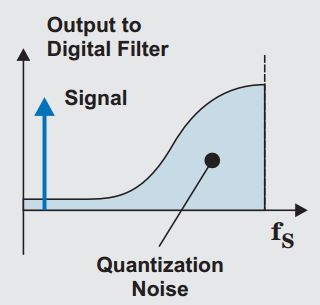
\includegraphics[width=0.40\textwidth, height = 4cm]{modeladoderuido}
  \caption{Ilustracion sobre como el modelado de ruido empuja las frecuencias de ruido a bandas que no perjudican a la medicion}\label{fig:modeladoderuido}
\end{figure}

% subsubsection el_modulador_delta_sigma (end)

\subsubsection{El filtro digital y filtro de decimacion} % (fold)
\label{ssub:el_filtro_digital_y_filtro_de_decimacion}

Una vez que la señal esta en el dominio digital, un filtro pasa-bajos digital se encarga de eliminar el ruido en alta frecuencia, y un filtro de decimacion se utiliza para disminuir la frecuencia de datos a la salida del conversor. \\

El filtro digital se implementa tomando las muestras del tren de pulsos de 1 bit y ponderando las muestras en un promedio. La frecuencia de salida del filtro digital es la misma que la frecuencia de muestreo. La Figura \ref{fig:filtrodigital} muestra la salida del filtro en el dominio del tiempo y de la frecuencia. En el dominio del tiempo, puede verse que la salida de la señal se corresponde con la entrada analógica, que corresponde a una función seno. En el dominio de la frecuencia, puede verse como el ruido fue reducido por el filtro digital. La salida de este filtro es una onda muy parecida a la entrante, a una frecuencia alta. La cantidad de información es demasiada y no es necesaria. Por esto es que se aplica, luego del filtro digital, el filtro de decimacion. \\

\begin{figure}[h]
  \centering
  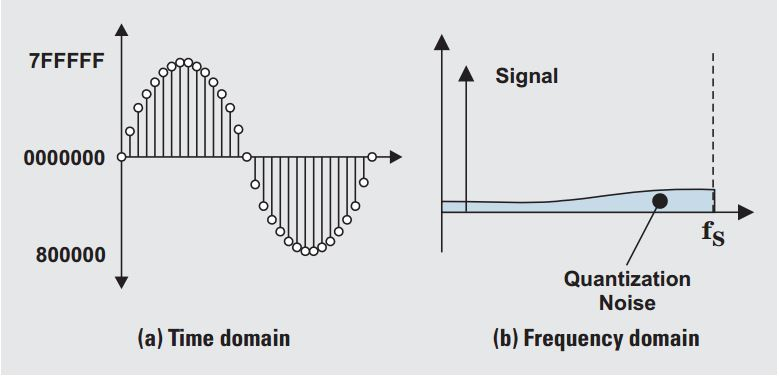
\includegraphics[width=0.80\textwidth, height = 6.3cm]{filtrodigital}
  \caption{Salida del filtro digital en el dominio del tiempo y de la frecuencia.}\label{fig:filtrodigital}
\end{figure}

El filtro de decimacion selecciona algunos datos de la señal de salida del filtro digital y descarta otros. La frecuencia de selección se denomina frecuencia de datos $f_s$ y es la frecuencia de salida del conversor. A pesar de que se elimina información, hay que recordar que no se elimina tanto como para no poder tener todos los datos necesarios acerca de la señal de entrada. Con el teorema de Nyquist\cite{shannon}, es posible reconstruir la señal de entrada sin perder información. La Figura \ref{fig:decimacion} muestra el proceso de decimacion.\cite{delta_sigma_2} %http://lavryengineering.com/pdfs/lavry-sampling-theory.pdf

\begin{figure}[h]
  \centering
  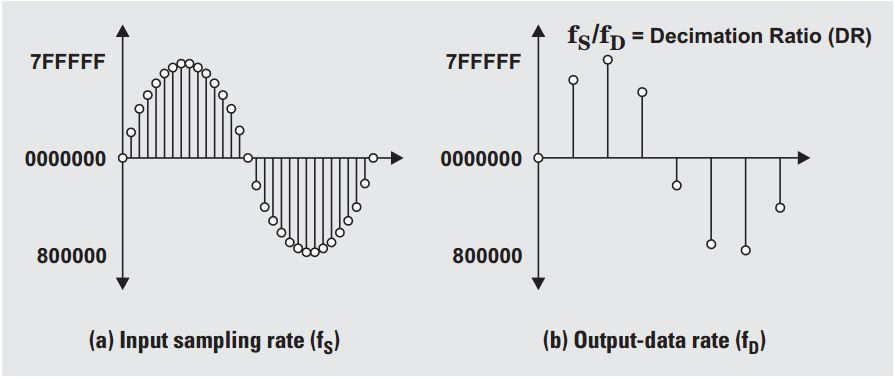
\includegraphics[width=0.80\textwidth, height = 6.3cm]{decimacion}
  \caption{Entrada (a) y salida (b) de la señal procesada por el filtro de decimacion. }\label{fig:decimacion}
\end{figure} 

% subsubsection el_filtro_digital_y_filtro_de_decimacion (end)


% subsection conversor_delta_sigma (end)

\section{Amplificadores de Instrumentación} %fold
\label{sec:amplificadores_de_instrumentacion}

%Bib: INSTRUMENTACIÓN ELECTRÓNICA DE COMUNICACIONES. José María Drake Moyano. UNIVERSIDAD DE CANTABRIA 2005.
%Bib: Apuntes de Clases, Electrónica 2. Universidad Nacional de Rosario Facultad de Ciencias Exactas, Ingeniería y Agrimensura Escuela de Ingeniería Electrónica.
%Bib: A Designer’s Guide to Instrumentation Amplifiers. 2da Edition, Charles Kitchin and Lew Count.

Los amplificadores de instrumentación surgen ante la necesidad de medir tensiones de muy bajo nivel, eliminando señales de interferencias e indeseadas (ruido) en modo común.
Se denomina amplificador de instrumentación a todo dispositivo creado a partir de amplificadores operacionales. Su diseño incluye:

\begin{itemize}
  \item Alta impedancia de entrada
    \item Alto rechazo de modo común
    \item Ganancia estable y variable con una única resistencia y que no se contraponga directamente la ganancia con el ancho de banda (fenómeno que suele suceder en los amplificadores operacionales).
\end{itemize}

Además está hecho con tensiones y corrientes de desequilibrio (offset) bajas y con pocas derivas e impedancia de salida baja.

En el circuito de la Figura \ref{fig:aibasico} puede verse el esquema clásico para la realización de un amplificador de instrumentación, donde se ha colocado el circuito equivalente de la fuente de señal.

\begin{figure}[h]
  \centering
  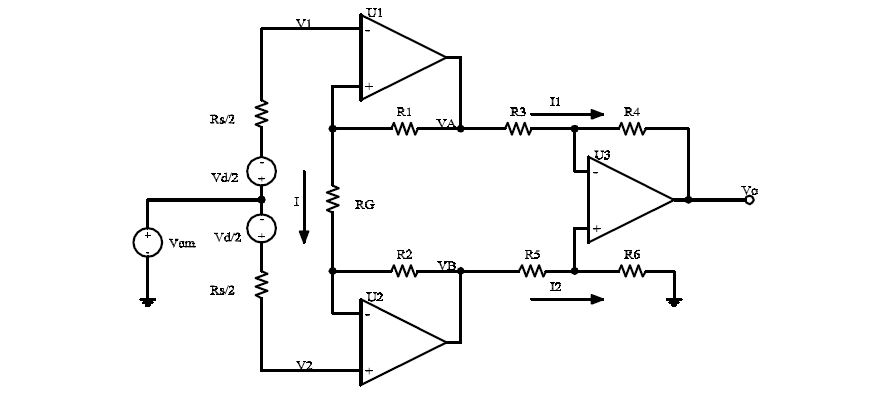
\includegraphics[width=0.60\textwidth, height = 4cm]{ai1}
  \caption{Amplificador Instrumental Básico}\label{fig:aibasico}
\end{figure}

El circuito está formado por una primera etapa con salida y entrada diferencial de alta impedancia, que amplifica únicamente la tensión diferencial de entrada; la segunda etapa es un amplificador diferencial con salida unipolar y ganancia en modo común nula idealmente.

Suponiendo amplificadores operacionales ideales: 

\begin{equation}\label{eq1}
I = \frac{V_1 - V_2}{R_g}  => \frac{R_1+R_2+R_g}{R_g} (V_d)
\end{equation}

Como la segunda etapa es un diferencial, si suponemos (R\textsubscript{3}R\textsubscript{6}=R\textsubscript{4}R\textsubscript{5}) y  (R\textsubscript{1}=R\textsubscript{2}) resulta la siguiente expresión de la tensión de salida:

\begin{equation}\label{eq2}
V_0 = \frac{R_6}{R_5}(1 +\frac{2R_1}{R_g} (V_d))
\end{equation}

En la segunda etapa:

\begin{equation}\label{eq3}
V_{cm}|_{2etapa} = \frac{V_A + V_B}{2}=V_{cm} +\frac{R_2 - R_1}{2R_g}(V_d)
\end{equation}

Podemos ver que la tensión en modo común vista por la segunda etapa es la misma que en la entrada mas un termino que depende de la tensión diferencial, producida por una variación del modo común en función de la tensión de entrada.

Entonces se llegan a las siguientes conclusiones:
\begin{enumerate}
\item La ganancia al modo común de la primera etapa es la unidad, siendo sus funciones:
\begin{itemize}
\item Amplificar la tensión diferencial.
\item Proporcionar un ajuste cómodo de la ganancia mediante R\textsubscript{g}.
\item Presentar una elevada impedancia de entrada.
\end{itemize}
\item El CMR (rechazo del modo común) depende del que presente la etapa diferencial de salida, y de la ganancia diferencial de la primera etapa.
\end{enumerate}

\subsection{Características de entrada de un Amplificador de Instrumentación} %fold
\label{sec:caract_entrada_amplificadores}
Evidentemente es deseable aproximarse al máximo a las características del amplificador de instrumentación ideal, se mostrará las características no ideales de estos dispositivos, considerando el modelo de amplificador de instrumentación real de la Figura \ref{fig:aireal}.

\begin{figure}[h]
  \centering
  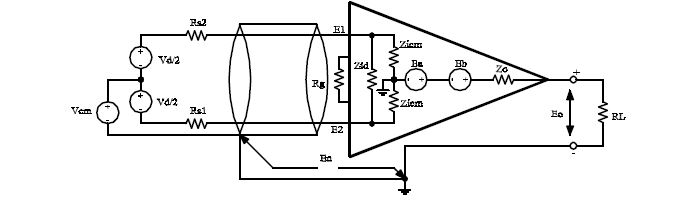
\includegraphics[width=1.0\textwidth, height = 4cm]{ai2}
  \caption{Modelo de un amplificador de instrumentación real.}\label{fig:aireal}
\end{figure}

\subsubsection{Impedancia de Entrada} %fold
\label{impedancia_entrada}
Si consideramos que las impedancias de entrada son infinitas, entonces debería existir un error en la ganancia efectiva debido a la resistencia de salida de la fuente.

La impedancia Z\textsubscript{id} representa la impedancia de entrada diferencial, que depende de R\textsubscript{g} y por eso también de la ganancia diferencial.

La impedancia de entrada en modo común Z\textsubscript{icm} está representada por dos componentes iguales entre cada entrada y masa. Esta impedancia puede haber sido medida de dos formas:

\begin{itemize}
\item Como la existente entre cada entrada por separado y masa, siendo entonces su representación en el circuito equivalente a la mostrada en la Figura \ref{fig:aireal}.
\item Como la medida entre las dos entradas cortocircuitadas y masa. En este método obtendremos evidentemente la mitad que en la anterior.
\end{itemize}

La impedancia de entrada diferencial, debido a la resistencia de salida de la fuente de señal, nos va a producir una pérdida de ganancia. El error de ganancia supuesto R\textsubscript{s}=R\textsubscript{s1}+R\textsubscript{s2}, tendrá el valor:

\begin{equation}\label{eq4}
1 - \frac{Z_{id}}{Z_{id}+R_{s}}= \frac{R_{s}}{Z_{id}+R_{s}}
\end{equation}

Debemos tener en cuenta que el Z\textsubscript{icm} sea igual en las dos entradas, y que las resistencias de salidas de la fuente de señal también sean iguales, sino la señal se dividirá de manera desigual en las dos entradas produciendo una tensión diferencial, debido al modo común, no pudiendo separar la señal que si se quiere amplificar. Si se produce esta tensión diferencial se vería deteriorado sensiblemente el CMR del circuito.

%subsubsection impedancia_entrada (end)

\subsubsection{No Linealidad} %fold
\label{no_linealidad}

La linealidad de la función de transferencia de un amplificador se mide
respecto al caso ideal que correspondería con una función de transferencia constituida
por una recta, tal y como se representa en la Figura \ref{fig:linealidad}.

\begin{figure}[h]
  \centering
  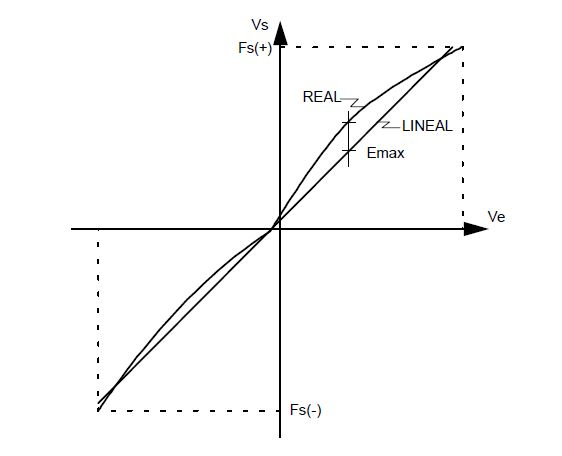
\includegraphics[width=0.60\textwidth, height = 4cm]{ai4}
  \caption{No linealidad de la función de transferencia de un amplificador de instrumentación.}\label{fig:linealidad}
\end{figure}

Existen varias definiciones de linealidad según la recta que consideremos. Nosotros vamos a usar la recta que mejor se adapte a la función de transferencia del amplificador, que suele ser la utilizada por los fabricantes cuando nos dan la linealidad de un AI integrado. Esta recta no tiene por qué pasar por el origen, ni presentar la pendiente marcada por la ganancia esperada del AI. Tiene que ser aquella que nos de el menor valor de no linealidad (NL), definida como:

\begin{equation}\label{eq5}
NL = \frac{|Salida Real - Salida lineal|_{max}}{Margen de variación de la salida entre fondos de escala}
\end{equation}

%subsubsection no_linealidad (end)

\subsubsection{Rechazo al Modo Común} %fold
\label{rechazo_CMR}

Como se ve en la Figura \ref{fig:aireal}, la tensión de salida tiene dos componentes. Uno de ellos es proporcional a la tensión de entrada diferencial y el otro a la tensión de modo común. La tensión de modo común que aparece entre los terminales de entrada del amplificador se define como: 

\begin{equation}\label{eq6}
E_{cm} = \frac{(E_{2}+E{1})}{2}
\end{equation}

Esta puede consistir en una cierta tensión de modo común de la fuente más cualquier tensión de ruido, E\textsubscript{n}, entre el común de la fuente y el del amplificador. La constante G\textsubscript{d} representa el factor de ganancia del amplificador diferencial (fijado por la resistencia exterior de selección de ganancia), mientras que la constante G\textsubscript{g}/CMR representa la ganancia al modo común del amplificador. El CMRR (relación de rechazo al modo común) está directamente relacionado con la ganancia diferencial y aumenta cuando lo hace esta. 

Idealmente deben seguir la misma progresión, es decir si G\textsubscript{d} aumenta 20 dB el CMRR debería aumentar 20dB (suponiendo que G\textsubscript{cm} se mantiene constante); pero en los circuitos reales esto no se cumple y el aumento de CMRR es menor. Se expresa habitualmente para los valores máximo y mínimo de la ganancia del amplificador y se mide en decibelios.

%subsection rechazo_CMR (end)

\subsubsection{Tensión de Offset} %fold
\label{tension_off}
La mayoría de los Amplificadores de Instrumentación son dispositivos de dos etapas: tienen una etapa de entrada de ganancia variable y otra de salida de ganancia fija. Por lo tanto podemos definir los siguientes parámetros:

\begin{itemize}
\item V\textsubscript{IOS} (Tensión de offset de la etapa de entrada): Es la tensión que debe aplicarse a la entrada de la etapa de entrada para forzar que su salida sea nula.
\item V\textsubscript{OOS} (Tensión offset de la etapa de salida) : Es la tensión que deberá aplicarse, en el caso de que sea accesible, a la entrada de la etapa de salida para producir una salida de cero voltios.
\item  V\textsubscript{OS} (Tensión offset global) : Es la tensión total de offset, referida a la entrada. Considerando que la etapa de entrada es la que presenta la ganancia diferencial del amplificador de instrumentación (a la segunda etapa se le suele asignar la unidad), la expresión del voltaje offset total será la siguiente:

\begin{equation}\label{eq7}
V_{OS} = V_{IOS} + \frac{V_{OOS}}{G_d}
\end{equation}

Podemos ver que a la salida tendremos un offset total de V\textsubscript{OOS} G\textsubscript{d}.
\end{itemize}

%subsubsection tension_off (end)

%subsection caract_entrada_amplificadores (end)

\subsection{Amplificadores de Instrumentación con Ganancia Programable} %fold
\label{ganancia_programable}

Se pueden incorporan en los montajes de los amplificadores de instrumentación una red de resistencias seleccionables digitalmente, para hacer las veces de R\textsubscript{G} y así poder cambiar el valor de la ganancia mediante un control digital, desde por ejemplo el sistema de adquisición de datos, constituyendo lo que se denomina amplificador de instrumentación de ganancia programable. Un amplificador de este tipo se puede realizar mediante componentes
discretos, utilizando resistencias y puertas analógicas, pero las características obtenidas serán, en la mayoría de las ocasiones, sensiblemente inferiores a las de los dispositivos integrados.

En la Figura \ref{fig:programable}  se puede ver el esquema del amplificador de instrumentación con ganancia programable PGA206/207 de Burr-Brown. La ganancia de este amplificador se puede controlar por medio de las entradas A1 y A2 para conseguir ganancias de 1, 2, 4 u 8.

\begin{figure}[h]
  \centering
  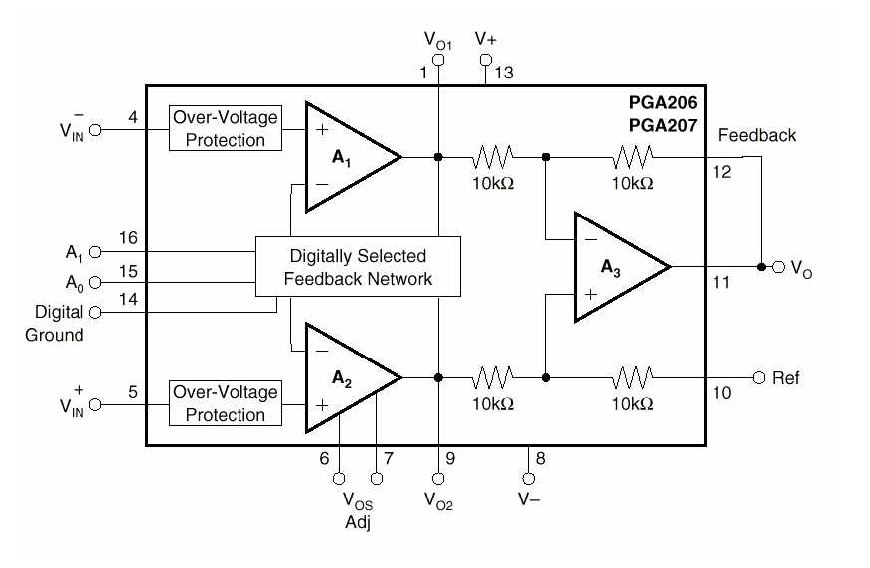
\includegraphics[width=1.0\textwidth, height = 7cm]{ai5}
  \caption{Amplificador de Instrumentación programable PGA206.}\label{fig:programable}
\end{figure}

En este modelo las entradas analógicas están protegidas contra sobre-tensiones de hasta 40 voltios, incluso sin alimentación. Las resistencias internas están ajustadas por láser para conseguir una baja tensión de offset y pequeñas derivas.

La entrada puede provenir de un sistema multicanal multiplexado puesto que el amplificador tiene un tiempo de asentamiento muy corto. Además las entradas tipo FET eliminan los errores debidos a la corriente de polarización y a la resistencia parásita serie asociada a los multiplexores analógicos.


% subsection ganancia_programable (end)

%section amplificadores_de_instrumentacion (end)

\section{Sistema de control para motor sin escobillas} % (fold)
\label{sec:sistema_de_control_para_motor_sin_escobillas}

%Bib : Control motor brushless sensorless. Trabajo de Fin de Grado. Gonzalo Solchaga y Jesus Maria Corres Sanz. Junio 2015.
%Bib : Desarrollo de un controlador para motores DC brushless basado en CompactRIO y LabVIEW de National Instruments para el estudio de nuevos algoritmos de control.Proyecto fin de carrera. Juan Miguel Garcia Haro. 2011
%Bib: http://www.digikey.com/en/articles/techzone/2013/mar/an-introduction-to-brushless-dc-motor-control

\subsection{Motor DC sin escobillas (Motores Brushless)}
\label{subsec: motor_sin_escobillas}

Los motores DC brushless no emplean escobillas en la conmutación para la transferencia de energía, estas producen rozamiento, disminuyen el rendimiento, generan calor, son ruidosos y demandan una sustitución periódica y, por tanto, un mayor mantenimiento.

Algunas de las ventajas de los motores BLDC con respecto a los motores DC convencionales son:

\begin{itemize}
\item Mejor relación velocidad-par motor.
\item Mayor respuesta dinámica.
\item Mayor eficiencia.
\item Menor ruido
\item Mayor vida útil.
\item Mayor rango de velocidad.
\item Mejor relación par motor - tamaño (por lo que son mejores en para los espacios reducidos).
\end{itemize}

%subsection sistemas_sin_escobillas (end)

\subsection{Clasificación de Motores sin Escobillas}
\label{clasificacion_motores}

Los motores DC Brushless se clasifican en dos: 

\begin{enumerate}
\item Inrunner.
\item Outrunner.
\end{enumerate}

Los Inrunner desarrollan mayor velocidad y suelen ser mas pequeños, entregan su máximo torque a muy altas revoluciones por minuto (RPM), por lo que se usan siempre con engranajes reductores. En estos motores el elemento móvil es el eje, sobre el cual se encuentran instalados los imanes permanentes.

Los motores Outrunner desarrollan su torque máximo a velocidades mas bajas, por lo que usualmente no necesitan reducción, y se pueden acoplar directamente a una hélice. En estos los imanes permanentes están instalados en la carcasa externa del motor, que en este caso es la que gira y el bobinado se encuentra fijado al eje.

Estos motores trabajan por medio de variadores, también llamados controladores de velocidad (electronic speed controler o ESC), que transforman la corriente continua de las baterías en una tensión alterna trifásica y la alimentan a los bobinados en cierta secuencia dependiendo de la posición del rotor.
Para manejar los motores se precisa el conocimiento de la posición del rotor en cada momento, para lo cual se utilizan dos técnicas básicamente, dependiendo de la existencia o no de sensores en el motor, lo que los divide en dos familias: con sensores (sensored) y sin sensores (sensorless).

\begin{itemize}
  \item Con sensores: Disponen de sensores de efecto hall o de encoders que indican la posición del rotor. Es habitual que tengan 3 sensores separados 120\textsuperscript{o}, uno para cada bobinado del motor.
  \item Sin sensores: No tienen sensores; la posición se determina mediante la medición del efecto de la fuerza contra-electromotriz sobre las bobinas
\end{itemize}





%subsection clasificacion_motores (end)

\subsection{Métodos de Control de Motores sin Escobillas}
\label{subsection: metodos_control_motores}

Los sistemas utilizados para el control con sensores se clasifican según el algoritmo utilizado. Los mas utilizados son los siguientes: 

\begin{itemize}
\item Conmutación trapezoidal o "six step mode".
\item Conmutación sinusoidal.
\item Control vectorial o Field Oriented Control.
\end{itemize}

\subsubsection{Conmutación trapezoidal}
\label{conmutacion_trapezoidal}

Es el método más simple de control de los motores sin escobillas. En este esquema se controla la corriente que circula por los terminales del motor, excitando un par simultáneamente y manteniendo el tercer terminal desconectado. Sucesivamente se va alternando el par de terminales a excitar hasta completar las seis combinaciones posibles. Las seis direcciones de las corrientes se muestran en la Figura \ref{fig:trapezoidal}

\begin{figure}[h]
  \centering
  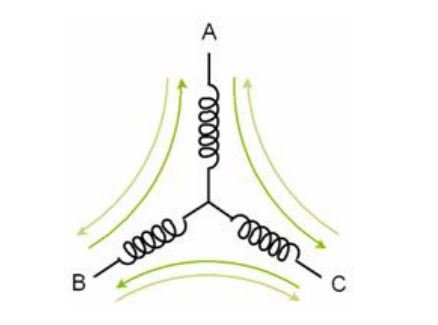
\includegraphics[width=1.0\textwidth, height = 7cm]{m1}
  \caption{Esquema de las seis posibles direcciones de circulación de corriente.}\label{fig:trapezoidal}
\end{figure}

Tiene como ventajas su sencillez y facilidad de implementación por lo cual es el método más usado en motores pequeños. Pese a esto, tiene un problema inherente a la conmutación del vector de corrientes que es un rizado en el torque de salida. En aplicaciones donde se requieren fuerzas uniformes o bajas velocidades, esto puede llegar a ser inconveniente. En la Figura \ref{fig:corrientes_bobinas} se muestran las corrientes por cada una de las fases, la secuencia de conmutación y el torque.

\begin{figure}[h]
  \centering
  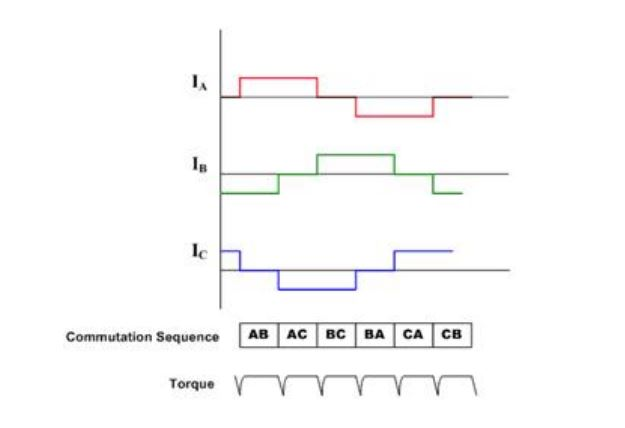
\includegraphics[width=1.0\textwidth, height = 7cm]{m2}
  \caption{: Corrientes en las bobinas y torque del motor.}\label{fig:corrientes_bobinas}
\end{figure}

\cite{brushless_control}

%subsubsection conmutacion_trapezoidal (end)

\subsubsection{Conmutación Sinusoidal}
\label{subsubsection: conmutacion_sin}

Es un método de control mas eficiente que el la conmutación trapezoidal, ya que intenta controlar la posición del rotor en continuamente.

Esta continuidad se consigue aplicando simultáneamente tres corrientes sinusoidales
desfasadas 120\textsuperscript{o} a los tres bobinados del motor. La fase de estas corrientes se escoge de forma que el vector de corrientes resultante siempre esté en cuadratura con la orientación del rotor y tenga un valor constante.

Como consecuencia de este procedimiento se obtiene un par más preciso y sin el rizado típico de la conmutación trapezoidal. No obstante, para poder generar dicha modulación sinusoidal es necesaria una medida precisa de la posición del rotor, que difícilmente se logra con sensores de efecto Hall, por lo cual se requiere de un encoder absoluto de alta resolución.

A bajas velocidades este método de control presenta el mejor desempeño en eficiencia y suavidad del torque, sin embargo a altas frecuencias no responde tan bien debido a la necesidad de procesar señales sinusoidales de frecuencias altas y a que los controladores PI usados para generar estas señales tienen una respuesta limitada en ganancia y frecuencia. Cuando la frecuencia es suficientemente alta, la eficiencia decrece y el error aumenta, tendiendo a un punto de cero torque.
%subsubsection conmutacion_sin (end)

\subsubsection{Control Vectorial}
\label{subsubsection: control_vectorial}

El problema principal que presenta la conmutación sinusoidal es que intenta controlar directamente las corrientes que circulan por el motor, las cuales son intrínsecamente variantes en el tiempo. Al aumentar la velocidad del motor, y por tanto la frecuencia de las corrientes, empiezan a aparecer problemas.

\begin{figure}[h]
  \centering
  \includegraphics[width=1.0\textwidth, height = 7cm]{control_vectorial}
  \caption{: Diagrama de Bloques del Control Vectorial.}\label{fig:control_vectorial}
\end{figure}

El control vectorial o Field Oriented Control (FOC) soluciona el problema controlando el vector de corrientes directamente en un espacio de referencia ortogonal y rotacional, llamado espacio D-Q (Direct - Quadrature) como se muestra en la Figura . Dicho
espacio de referencia está normalmente alineado con en el rotor de forma que permite que el control del flujo y del par del motor se realice de forma independiente. La componente directa permite controlar el flujo y la componente en cuadratura el par. Para este fin se requiere no solamente una muy buena medición de la orientación del rotor, sino un tratamiento matemático previo de las señales para transformarlas del marco trifásico estático de los bobinados en el estator (circuito fijo dentro del cual gira el rotor) al marco rotacional D-Q del rotor. Este es el control que presenta mejor respuesta en todos los rangos de velocidad pero resulta ser el más costoso de implementar, lo cual lo hace inadecuado para toda aplicación en la que no sea estrictamente necesario.

%subsubsection control_vectorial (end)

%subsection metodos_control_motores (end)


\pagebreak

\subsubsection{Banco de Ensayos para Motores}
\label{subsubsection: banco_ensayos}

%Bib: Proyecto de Fin de Carrera."Sistemas de adquisición de datos y control en tiempo real para bancos de ensayos de motores". Rodriguez Luis Gustavo y Maffei Ignacio.

El siguiente extracto está basado en la tesis de Rodriguez Luis Gustavo y Maffei Ignacio, "Sistemas de adquisición de datos y control en tiempo real para bancos de ensayos de motores", realizada en el Laboratorio de Arquitectura de Computadoras (LAC), Facultad de Ciencias Exactas Físicas y Naturales, UNC.

Para realizar ensayos a un motor es necesario instalarlo en un banco de pruebas o de ensayos. Este consta básicamente de los siguientes elementos:

\begin{itemize}
\item Cimentación: absorbe las vibraciones que se producen debido a la existencia en el motor de fuerzas de inercia no equilibradas y de los correspondientes momentos resultantes.
\item Bancada: soporta el motor ensayado.
\item Soporte: permite montar y fijar el motor en la bancada, así como regular la altura y alinear el motor con el freno.
\item Freno dinamométrico: absorbe la potencia desarrollada por el motor, ofreciendo una resistencia al giro de éste, y debe estar provisto de dispositivo para medir el par motor.
\item Eje de Transmisión: Permite la unión mecánica del freno con el motor, con una cierta elasticidad y capacidad de absorber desalineaciones.
\item Amortiguador torsional: su función es de amortiguar el movimiento alternativo del motor y las vibraciones del motor para que no influyan en el dinamómetro.
\item Sistema de combustible: se debe suministrar el combustible al motor mediante cañerías directo desde un tanque de combustible o a través de los instrumentos de medición de consumo.
\item Sistema de refrigeración del motor: si los motores son refrigerados por agua, normalmente se utiliza la bomba de agua del propio motor. Esta impulsa el agua a través del motor hacia un intercambiador de calor (agua/agua o agua/aire), en general con regulación termostática por medio de válvulas.
Si los motores son refrigerados por aire se suele utilizar un ventilador dirigido hacia las aletas del motor.
\item Sistema de refrigeración de aceite: en ocasiones también se refrigera el aceite del motor, ya que al no existir una corriente de aire al cárter, éste tiende a sobre-calentarse. El sistema consta de un intercambiador aceite/agua y en ocasiones una bomba auxiliar.
\item Sistema de refrigeración del dinamómetro: los frenos dinamométricos por corrientes de Foucault y los hidráulicos transforman toda la energía mecánica que reciben del motor en calor. Este calor es eliminado por el sistema de refrigeración del freno, que suele ser mediante el abastecimiento continuo de agua a través de un circuito cerrado.
\item Red de agua: es un circuito cerrado cuya función es disminuir la temperatura del agua proveniente del dinamómetro y del intercambiador de calor del agua y aceite del motor.
\item Sistema de ventilación de la sala: se debe evitar el sobrecalentamiento de la sala por la radiación de calor del motor. Se efectúa mediante ventiladores axiales o centrífugos de impulsión y extracción.
\item Sistema de evacuación de los gases de escape del motor: los gases de escape deben ser enviados a la atmósfera, tras pasar por una cámara de expansión.
\item Sistema de arranque: este sistema permite poner en marcha el motor a ensayar sin necesidad de contar con el motor de arranque original del motor.
\item Elementos de medición: los elementos principales de medición son:

\begin{itemize}
\item Taquímetro: mide la velocidad angular del motor (rpm).
\item Celda de carga: mide el torque ejercido por el motor.
\item Sensor temperatura de motor y del dinamómetro.
\item Sensor presión de aceite del motor y del dinamómetro.
\item Sensor de temperatura, presión, y humedad ambiente.
\item Caudalímetro de aire y combustible.
\item Sensores de otras temperaturas y presiones.
\item etc.
\end{itemize}

\end{itemize}

%subsection banco_ensayos (end)

% section sistema_de_control_para_motor_sin_escobillas (end)

\section{Sistemas de comunicación serie con inmunidad al ruido} % (fold)
\label{sec:sistemas_de_comunicacion_serie_con_inmunidad_al_ruido}

%CITADO

\subsection{Comunicacion serial} % (fold)
\label{sub:comunicacion_serial}
%que es la comunicacion serial? http://digital.ni.com/public.nsf/allkb/039001258CEF8FB686256E0F005888D1

La comunicación serial es un protocolo de comunicación de transmisión asincrónica entre dispositivos, que se incluye de manera estándar en prácticamente cualquier computadora. La mayoría de las computadoras incluyen dos puertos seriales RS-232. La comunicación serial es también un protocolo común utilizado por varios dispositivos para instrumentación; existen varios dispositivos compatibles con GPIB que incluyen un puerto RS-232. Además, la comunicación serial puede ser utilizada para adquisición de datos si se usa en conjunto con un dispositivo remoto de muestreo.

El concepto de comunicación serial es sencillo. El puerto serial envía y recibe bytes de información un bit a la vez. Aun y cuando esto es más lento que la comunicación en paralelo, que permite la transmisión de un byte completo por vez, este método de comunicación es más sencillo y puede alcanzar mayores distancias. Por ejemplo, la especificación IEEE 488 para la comunicación en paralelo determina que el largo del cable para el equipo no puede ser mayor a 20 metros, con no más de 2 metros entre cualesquier dos dispositivos; por el otro lado, utilizando comunicación serial el largo del cable puede llegar a los 1200 metros.

Típicamente, la comunicación serial se utiliza para transmitir datos en formato ASCII. Para realizar la comunicación se utilizan 3 líneas de transmisión: Tierra (o referencia), Transmitir, Recibir. Debido a que la transmisión es asincrónica, es posible enviar datos por un línea mientras se reciben datos por otra. Existen otras líneas disponibles para realizar handshaking, o intercambio de pulsos de sincronización, pero no son requeridas. Las características más importantes de la comunicación serial son la velocidad de transmisión, los bits de datos, los bits de parada, y la paridad. Para que dos puertos se puedan comunicar, es necesario que las características sean iguales.\cite{intro_serial}

\subsubsection{Conceptos} % (fold)
\label{ssub:conceptos}

\begin{itemize}
  \item \textbf{Velocidad de transmisión (baud rate):} Indica el número de bits por segundo que se transfieren, y se mide en baudios. Por ejemplo, 300 baudios representa 300 bits por segundo. Cuando se hace referencia a los ciclos de reloj se está hablando de la velocidad de transmisión. Por ejemplo, si el protocolo hace una llamada a 4800 ciclos de reloj, entonces el reloj está corriendo a 4800 Hz, lo que significa que el puerto serial está muestreando las líneas de transmisión a 4800 Hz. Las velocidades de transmisión más comunes para las lineas telefónicas son de 14400, 28800, y 33600. Es posible tener velocidades más altas, pero se reduciría la distancia máxima posible entre los dispositivos. Las altas velocidades se utilizan cuando los dispositivos se encuentran uno junto al otro, como es el caso de dispositivos GPIB.
  \item \textbf{Bits de datos:} Se refiere a la cantidad de bits en la transmisión. Cuando la computadora envía un paquete de información, el tamaño de ese paquete no necesariamente será de 8 bits. Las cantidades más comunes de bits por paquete son 5, 7 y 8 bits. El número de bits que se envía depende en el tipo de información que se transfiere. Por ejemplo, el ASCII estándar tiene un rango de 0 a 127, es decir, utiliza 7 bits; para ASCII extendido es de 0 a 255, lo que utiliza 8 bits. Si el tipo de datos que se está transfiriendo es texto simple (ASCII estándar), entonces es suficiente con utilizar 7 bits por paquete para la comunicación. Un paquete se refiere a una transferencia de byte, incluyendo los bits de inicio/parada, bits de datos, y paridad. Debido a que el número actual de bits depende en el protocolo que se seleccione, el término paquete se usar para referirse a todos los casos.
  \item \textbf{Bits de parada:} Usado para indicar el fin de la comunicación de un solo paquete. Los valores típicos son 1, 1.5 o 2 bits. Debido a la manera como se transfiere la información a través de las líneas de comunicación y que cada dispositivo tiene su propio reloj, es posible que los dos dispositivos no estén sincronizados. Por lo tanto, los bits de parada no sólo indican el fin de la transmisión sino además dan un margen de tolerancia para esa diferencia de los relojes. Mientras más bits de parada se usen, mayor será la tolerancia a la sincronía de los relojes, sin embargo la transmisión será más lenta.
  \item \textbf{Paridad:} Es una forma sencilla de verificar si hay errores en la transmisión serial. Existen cuatro tipos de paridad: par, impar, marcada y espaciada. La opción de no usar paridad alguna también está disponible. Para paridad par e impar, el puerto serial fijará el bit de paridad (el último bit después de los bits de datos) a un valor para asegurarse que la transmisión tenga un número par o impar de bits en estado alto lógico. Por ejemplo, si la información a transmitir es 011 y la paridad es par, el bit de paridad sería 0 para mantener el número de bits en estado alto lógico como par. Si la paridad seleccionada fuera impar, entonces el bit de paridad sería 1, para tener 3 bits en estado alto lógico. La paridad marcada y espaciada en realidad no verifican el estado de los bits de datos; simplemente fija el bit de paridad en estado lógico alto para la marcada, y en estado lógico bajo para la espaciada. Esto permite al dispositivo receptor conocer de antemano el estado de un bit, lo que serviría para determinar si hay ruido que esté afectando de manera negativa la transmisión de los datos, o si los relojes de los dispositivos no están sincronizados.
\end{itemize}\cite{intro_serial}

% subsubsection conceptos (end)

% subsection comunicacion_serial (end)

\subsection{Implementando la inmunidad al ruido en comunicaciones seriales} % (fold)
\label{sub:implementando_la_inmunidad_al_ruido_en_comunicaciones_seriales}

En un sistema complejo, puede existir ruido proveniente de varias fuentes distintas. Esto incluye al ruido del ambiente, como el de la fuente de alimentación, etcétera. Las fuentes que producen ruido presentan una amenaza a fallos de datos en una comunicación serial. En esta sección se mencionan diversas técnicas aplicables a la tecnología de comunicación serial, que disminuyen el ruido presente, disminuyendo la tasa de errores.\cite{ruido_serial}

\begin{itemize}
  \item \textbf{Filtro RC externo:} Un filtro RC pasa-bajos externo es una manera de inmunizar el sistema al ruido en altas frecuencias, pero presenta el problema de empeorar la velocidad de los flancos de subida en el canal de comunicación y agrega una carga a los pines involucrados. Un flanco lento es mas susceptible al ruido y puede causar inestabilidad en el sistema. Para resultados óptimos, es necesario realizar un balance entre la reducción de ruido y la reducción en la velocidad del flanco. El balance se obtiene cambiando los valores de las resistencias involucradas en el filtro. Los valores dependerán del valor de reducción de ruido requerido y la tensión de alimentación
  \item \textbf{Fuente de alimentación desacoplada:} Hay ocasiones en las que el ruido proveniente de la fuente de alimentación puede causar errores en la comunicación. La reducción de este ruido se puede alcanzar utilizando filtros LC, también llamados ``Ferrite Beads''. Estos dispositivos son inductores hechos específicamente para ser colocados en serie con el cable de alimentación para reducir el ruido en alta frecuencia producido por la fuente. Típicamente, se suelen colocar capacitores de distintos valores luego del inductor para mejorar el filtrado. 
  \item \textbf{Filtros digitales:} También es posible utilizar filtros digitales para reducir ruido. Esto se suele ver sobretodo en diseño de sistemas FPGA. Los filtros digitales pueden ser realizados en VHDL o Verilog, y filtran tanto la señal de datos como la señal del clock. Los distintos parámetros del filtro están dados en la frecuencia de oscilación y el tiempo de filtrado deseado. 
\end{itemize}

% subsection implementando_la_inmunidad_al_ruido_en_comunicaciones_seriales (end)

% section sistemas_de_comunicacion_serie_con_inmunidad_al_ruido (end)

\section{Medición de frecuencia de RPM} % (fold)
\label{sec:medicion_de_frecuencia_de_rpm}
%CITADO

Un tacometro es un dispositivo digital que mide e indica la velocidad de un objeto en rotación. Un objeto en rotación puede ser un ventilador, la rueda de un auto, o cualquier cosa que esta en movimiento de revolución. Los tacometros digitales se pueden clasificar en cuatro tipos dependiendo de la técnica de adquisición de datos y la técnica de medición.

Basándose en la técnica de adquisición de datos, los tacometros digitales pueden ser de tipo:

\begin{itemize}
  \item \textbf{Con contacto:} El dispositivo de medición esta en contacto con la pieza de revolución que se utiliza para medir. 
  \item \textbf{Sin contacto:} El dispositivo de medición no esta conectado físicamente al motor. Se suele utilizar un láser para determinar la velocidad de la pieza de revolución
\end{itemize}

Basándose en la técnica de medición, pueden ser:

\begin{itemize}
  \item \textbf{Medición de tiempo:} Calcula la velocidad calculando el tiempo entre los pulsos medidos. Suelen ser mas precisos en velocidades bajas.
  \item \textbf{Medición de frecuencia:} Calcula la velocidad midiendo la frecuencia de los pulsos en un intervalo de tiempo. Suelen ser mas precisos en velocidades altas.
\end{itemize}

\subsection{Medición con fotointerruptor o sensor óptico} % (fold)
\label{sub:medicion_con_fotointerruptor_o_sensor_optico}
%http://www.utopiamechanicus.com/article/arduino-photo-interruptor-slotted-optical-switch/

Un fotointerruptor es un dispositivo que contiene dos extremos de los cuales de uno se emite luz y del otro se recibe mediante un fotosensor. En la Figura \ref{fig:fotointerruptor} se puede ver un ejemplo de uno de ellos. Con este dispositivo, es posible implementar un tacometro de adquisición sin contacto y medición de frecuencia.\cite{slotted_sensor}

\begin{figure}[h]
  \centering
  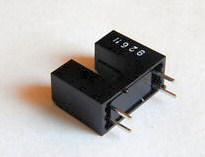
\includegraphics[width=0.20\textwidth, height = 3cm]{fotointerruptor}
  \caption{Fotointerruptor o sensor óptico}\label{fig:fotointerruptor}
\end{figure}

En el momento que el fotointerruptor esta conectado, se emite una luz infrarroja que va desde el lado emisor al receptor. Si se recibe luz, se genera una tensión (cuyo valor depende del fotointerruptor utilizado) en la salida del fotointerruptor, si no se recibe luz, se tienen 0 Volts a la salida. Un circuito típico puede verse en la Figura \ref{fig:circuitotipico_fotointerruptor} \\

\begin{figure}[h]
  \centering
  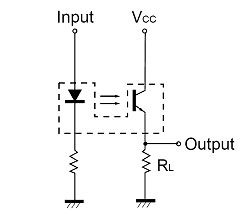
\includegraphics[width=0.30\textwidth, height = 5cm]{circuitotipico_fotointerruptor}
  \caption{Uso típico de un fotointerruptor}\label{fig:circuitotipico_fotointerruptor}
\end{figure}

Considerando el comportamiento de este dispositivo, es posible generar un generador de pulsos colocando algún objeto que obstruya el camino de la luz del fotointerruptor, y que esta obstrucción se de en cada vuelta del motor. Un ejemplo seria poner un aspa que gire con el eje, y que sea esta misma aspa la que obstruye la luz que va de un extremo a otro del fotointerruptor.

Esta señal de pulsos que sale del fotointerruptor puede servir como entrada a un microcontrolador que cuente los pulsos en un intervalo de tiempo, y así determinar la velocidad del motor.

% subsection medicion_con_fotointerruptor_o_sensor_optico (end)

% section medicion_de_frecuencia_de_rpm (end)

\section{Sistemas de base de datos para sistemas embebidos} % (fold)
\label{sec:sistemas_de_base_de_datos_para_sistemas_embebidos}

Una base de datos es un conjunto de datos pertenecientes a un mismo contexto y almacenados sistemáticamente para su posterior uso. En este sentido; una biblioteca puede considerarse una base de datos compuesta en su mayoría por documentos y textos impresos en papel e indexados para su consulta. Actualmente la mayoría de las bases de datos están en formato digital, siendo este un componente electrónico, y por ende se ha desarrollado y se ofrece un amplio rango de soluciones al problema del almacenamiento de datos.
Existen programas denominados sistemas gestores de bases de datos, abreviado DBMS, que permiten almacenar y posteriormente acceder a los datos de forma rápida y estructurada. Las propiedades de estos DBMS, así como su utilización y administración, se estudian dentro del ámbito de la informática.
MySQL es un sistema de gestión de base de datos muy conocido y muy usado actualmente. Existe una versión de MySQL para sistemas embebidos, denominada SQLite. 

\subsection{MySQL} % (fold)
\label{sub:mysql}

MySQL es un sistema de gestión de bases de datos relacional, multihilo y multiusuario. Está escrito en C y C++ y emplea el lenguaje SQL para consultas a la base de datos.
MySQL es muy utilizado en aplicaciones web, como Drupal o phpBB, en plataformas (Linux/Windows-Apache-MySQL-PHP/Perl/Python), y por herramientas de seguimiento de errores como Bugzilla. Su popularidad como aplicación web está muy ligada a PHP, que a menudo aparece en combinación con MySQL.
MySQL es una base de datos muy rápida en la lectura cuando utiliza el motor no transaccional MyISAM, pero puede provocar problemas de integridad en entornos de alta concurrencia en la modificación. En aplicaciones web hay baja concurrencia en la modificación de datos y en cambio el entorno es intensivo en lectura de datos, lo que hace a MySQL ideal para este tipo de aplicaciones. Sea cual sea el entorno en el que va a utilizar MySQL, es importante monitorizar de antemano el rendimiento para detectar y corregir errores tanto de SQL como de programación.


% subsection mysql (end)

\subsection{SQLite} % (fold)
\label{sub:sqlite}


SQLite es un sistema de gestión de bases de datos relacional compatible con ACID, contenida en una relativamente pequeña (~275 kiB) biblioteca escrita en C. 
A diferencia de los sistemas de gestión de bases de datos cliente-servidor, el motor de SQLite no es un proceso independiente con el que el programa principal se comunica. En lugar de eso, la biblioteca SQLite se enlaza con el programa pasando a ser parte integral del mismo. El programa utiliza la funcionalidad de SQLite a través de llamadas simples a subrutinas y funciones. Esto reduce la latencia en el acceso a la base de datos, debido a que las llamadas a funciones son más eficientes que la comunicación entre procesos. El conjunto de la base de datos (definiciones, tablas, índices, y los propios datos), son guardados como un sólo fichero estándar en la máquina host. Este diseño simple se logra bloqueando todo el fichero de base de datos al principio de cada transacción.
En su versión 3, SQLite permite bases de datos de hasta 2 Terabytes de tamaño, y también permite la inclusión de campos tipo BLOB. (10)

\subsubsection{Características} % (fold)
\label{ssub:caracteristicas}

La biblioteca implementa la mayor parte del estándar SQL-92, incluyendo transacciones de base de datos atómicas, consistencia de base de datos, aislamiento, y durabilidad (ACID), triggers y la mayor parte de las consultas complejas.
SQLite usa un sistema de tipos inusual. En lugar de asignar un tipo a una columna como en la mayor parte de los sistemas de bases de datos SQL, los tipos se asignan a los valores individuales. Por ejemplo, se puede insertar un string en una columna de tipo entero (a pesar de que SQLite tratará en primera instancia de convertir la cadena en un entero). Algunos usuarios consideran esto como una innovación que hace que la base de datos sea mucho más útil, sobre todo al ser utilizada desde un lenguaje de scripting de tipos dinámicos. Otros usuarios lo ven como un gran inconveniente, ya que la técnica no es portable a otras bases de datos SQL. SQLite no trataba de transformar los datos al tipo de la columna hasta la versión 3.
Varios procesos o hilos pueden acceder a la misma base de datos sin problemas. Varios accesos de lectura pueden ser servidos en paralelo. Un acceso de escritura sólo puede ser servido si no se está sirviendo ningún otro acceso concurrentemente. En caso contrario, el acceso de escritura falla devolviendo un código de error (o puede automáticamente reintentarse hasta que expira un tiempo de expiración configurable). Esta situación de acceso concurrente podría cambiar cuando se está trabajando con tablas temporales. Sin embargo, podría producirse un interbloqueo debido al multihilo. (11)

% subsubsection caracteristicas (end)
% subsection sqlite (end)

% section sistemas_de_base_de_datos_para_sistemas_embebidos (end)



% chapter marco_teorico (end)